\chapter{تخصیص منابع در شبکه های دسترسی رادیویی ابری دارای ظرفیت محدود در لینک \lr{fronthaul}}
%\thispagestyle{empty}
\section{مقدمه}
در این فصل، هدف تخصیص منابع در شبکه های  دسترسی رادیویی ابری است که برای دو حالت لینک فراسو و لینک فروسو در نظر گرفته شده است. در اینجا فرض بر این است که واحدهای رادیویی، به صورت توزیع شده و مشارکتی همانند \lr{MIMO}، پیام را دریافت و یا ارسال می کنند که شبکه های دسترسی رادیویی ابری با مشارکت توزیع شده را ایجاد می نمایند.
برای استفاده از مزایای سیستمهای \lr{C-RAN} و \lr{MIMO}، از سیستم \lr{MIMO C-RAN} به طور همزمان استفاده می گردد که منجر به بهبود نرخ و بازدهی انرژی \lr{EE} می گردد. با استفاده از سیستم های \lr{MIMO}، می توان به نرخ داده ی بیشتری رسید.\newline
برای در نظر گرفتن لینک عملی بین واحد کنترل و واحد رادیوییها، که \lr{Fronthaul} نامیده می شود، ظرفیت لینک \lr{Fronthaul} محدود در نظر گرفته می شود. بنابراین، سیگنالی که از لینک \lr{Fronthaul} عبور می کند نیاز به فشرده سازی دارد.

در ادامه مدل سیستم برای لینک فروسو و فراسو بیان می شود.
\begin{figure}
  \centering
    \includegraphics[width=\linewidth]{./fig/mydraw1}
  \caption{ساختار 
  \lr{C-RAN}
  در  لینک فروسو.
  }
  \label{fig:cr1}
\end{figure}
 فرض مسئله بر این است که سیستم به صورت چند آنتنه (\lr{MIMO})  می باشد و ظرفیت \lr{Fronthaul} محدود است. همچنین، سیستم دارای چندین خوشه یا سلول که در هر خوشه، تعدادی  واحد رادیویی و تعدادی کاربر قرار دارد\cite{EEcluster,jcluster}. هدف، بدست آوردن بیشینه بازدهی انرژی می باشد.\newline
 در حالت لینک فروسو، پیام، پیش کدگذاری شده است و سپس فشرده سازی بر روی آن صورت گرفته است و از طریق لینک \lr{Fronthaul} به واحد رادیویی منتقل می شود تا پیام را به کاربران ارسال کنند \cite{Fronthaul, ulSimeone, precodSimeone}
 .\newline
 در حالت لینک فراسو، سیگنال از کاربران به واحدهای رادیویی منتقل شده و سپس پیام فشرده شده و به دست واحد کنترل می رسد؛ تا با استفاده از روش های ترکیب کردن \LTRfootnote{combining}، پیام ارسالی کاربران بازیابی شود. 

\section{لینک فروسو}
در این بخش، لینک فروسو برای سیستم \lr{MIMO C-RAN} در نظر گرفته شده است که واحد کنترل، پیام را پیش کدگذاری کرده سپس سیگنال پیش کدگذاری شده را فشرده می کند. سیگنال فشرده شده ی نهایی توسط لینک \lr{Fronthaul} با ظرفیت محدود منتقل می گردد
\cite{dlsnr}.
\newline
فرض بر این است که واحدهای رادیویی و کاربران خوشه بندی شده اند به طوری که در هر خوشه تعدادی واحد رادیویی است که به کاربران موجود در آن خوشه، سرویس دهی می کنند.\newline
در این سیستم، فرستنده می بایست اطلاعات حالت کانال را بداند
(\lr{CSIT}). 
 از آنجایی که \lr{CSIT} با کمی خطا با ارسال پایلوت در لینک فراسو بدست می آید، به همین دلیل فرض در اینجا به این صورت است که تخمین \lr{CSIT}، همراه با خطای مشخص است. در واحد کنترل، از پیش کدگذاری از نوع \lr{MMSE} برای کاهش تداخل بین کاربران و بهبود عملکرد سیستم استفاده می گردد.\newline
همچنین، ابتدا نرخ قابل دسترسی را با توجه به ظرفیت محدود \lr{Fronthaul}، بدست می آوریم. سپس توان تخصیص داده را بهینه می کنیم تا \lr{EE} به مقدار بهینه ی خود برسد.\newline
در ادامه، ابتدا مدل سیستم و سپس نرخ قابل دسترسی بیان شده و مسئله ی تخصیص توان بررسی می گردد\cite{mkm}.
\subsection{مدل سیستم}
لینک فروسو سیستم \lr{MIMO C-RAN} شامل $R$  واحد رادیویی می باشد که $D$ کاربر تک آنتنه را سرویس می دهند.فرض بر این است که کاربران و واحدهای رادیویی، به 
 $S$
 تا خوشه تقسیم شده اند که $v$ امین خوشه،
 دارای $R_v$ واحد رادیویی است که ${D}_v$ کاربر را سرویس دهی می کنند\cite{EEcluster}.
 همچنین، فرض بر این است که
$j$
امین واحد رادیویی، در $v$امین خوشه، توسط لینک فیبر نوری با ظرفیت محدود $c_{r_{(v,j)}}$ به \lr{CU} متصل می گردد. در نتیجه داریم:
\begin{equation}
\begin{split}
\mathcal{R}_v= \{  r_{(v,i)} | 1 \leq i \leq {R}_v , i\in Z^+\}, \\
\mathcal{C}_{\mathcal{R}_v}= \{C_{r_{(v,j)}}| 1 \leq j \leq {R}_v , j\in Z^+\}, \\
\mathcal{D}_v= \{  d_{(v,k)} | 1 \leq k \leq {D}_v , k\in Z^+\},  \\
\end{split}
\end{equation} 
که
 $\mathcal{R}_v$، $\mathcal{C}_{\mathcal{R}_v}$
 و
  $\mathcal{D}_v$
 به ترتیب نشان دهنده ی دسته ی واحدهای رادیویی، دسته ی ظرفیت لینک \lr{Fronthaul} و دسته ی کاربران در $v$امین دسته ی خوشه می باشد.\newline
در واحد کنترل، ما روش فشرده سازی بعد از پیش کدگذاری و سپس ارسال را اعمال کرده ایم. هر کاربر همزمان تداخل بین خوشه ها و داخل یک خوشه را همزمان دریافت می کنند.
 \subsection{آنالیز نرخ قابل دسترس}
در این زیربخش، نرخ قابل دسترسی سیستم بررسی می گردد.
\begin{theorem}\label{t1}
 نرخ قابل دسترسی برای کاربر $d_{(s,k)}$ به صورت زیر می باشد:
\begin{equation}\label{e1}
\mathfrak{R}_{d_{(s,k)}} = B \log_2(1+\gamma_{d_{(s,k)}}),
\end{equation}
که $B$ پهنای باند کانال و $\gamma_{d_{(s,k)}}$ همان \lr{SINR} دریافتی $k$امین کاربر در $s$امین دسته ی خوشه است که به صورت زیر بیان می گردد.  
\begin{equation}\label{5}
\gamma_{d_{(s,k)}}= \frac{p_{d_{(s,k)}}|\boldsymbol{h}_{\mathcal{R}_s, d_{(s,k)}}^H \boldsymbol{w}_{\mathcal{R}_{s},d_{(s,k)}}|^2}{I_{d_{(s,k)}}+BN_0}.
\end{equation}
در فرمول \eqref{5}، 
$I_{d_{(s,k)}}$
نشان دهنده ی توان سیگنال تداخلی است.$BN_0$
نشان دهنده ی توان نویز است و
$\boldsymbol{h}_{\mathcal{R}_s, d_{(s,k)}}$ 
 نشان دهنده ی بردار کانال بین $k$امین کاربر و واحدهای رادیویی
 $s$
 امین دسته ی خوشه می باشد. همچنین 
 $\boldsymbol{w}_{\mathcal{R}_{s},d_{(s,k)}}$
 نشان دهنده ی بردار پیش کدگذاری استفاده شده در $s$امین دسته ی خوشه ها برای $k$امین کاربر می باشد. 
 $p_{d_{(s,k)}}$
 توان ارسالی واحدهای رادیویی است که به $k$امین کاربر در $s$امین دسته ی خوشه ارسال می گردد.
\end{theorem}
\begin{proof}
فرض کنید $\boldsymbol{y}_{\mathcal{D}_s}$ یک بردار
 $D_s \times 1$
باشد که نشان دهنده ی سیگنال دریافتی توسط دسته ای از کاربران در $s$
امین خوشه باشد که به صورت زیر بدست می آید.
\begin{equation} \label{1}
\boldsymbol{y}_{\mathcal{D}_s} = \sum_{v=1}^S \boldsymbol{H}^H_{\mathcal{R}_v,\mathcal{D}_s}\hat{\boldsymbol{x}}_{\mathcal{R}_v}+ \boldsymbol{z}_{\mathcal{D}_s},
\end{equation}
که   $\hat{\boldsymbol{x}}_{ \mathcal{R}_v} = [\hat{x}_{ r_{(v,1)}},...,\hat{ x}_{ r_{(v,\mathcal{R}_v)}}]^T \in \mathbb{C}^{{R}_v } $ 
بردار سمبل ارسالی خوشه ی  $v$ ام می باشد.\newline
 $\boldsymbol{z_{\mathcal{D}_s}} \backsim \mathcal{N}(0,N_0\boldsymbol{I}_{{D}_s})$ 
 نویز گوسی سفید اضافه شونده می باشد که دارای توان $N_0$
 و 
 $\boldsymbol{H}_{\mathcal{R}_v,\mathcal{D}_s}=\left[\boldsymbol{h}_{\mathcal{R}_v,d_{(s,1)}},\ldots,\boldsymbol{h}_{\mathcal{R}_v,d_{(s,\mathcal{D}_s)}}\right]^T  \in \mathbb{C}^{{R}_v\times {D}_s}$ 
 نشان دهنده ی ماتریس کانال بین واحدهای رادیویی دسته ی $\mathcal{R}_v$ و کاربران $\mathcal{D}_s$ می باشد.
 بردار کانال از واحدهای رادیویی خوشه ی  $v$ به $k$ امین کاربر در خوشه ی $s$ام  
 $\boldsymbol{h}_{\mathcal{R}_v,d_{(s,k)}}\in \mathbb{C}^{{R}_v}$
 به صورت زیر مدل می شود \cite{cellfree}
 \begin{equation}\label{channel}
\boldsymbol{h}_{\mathcal{R}_v,d_{(s,k)}} = \boldsymbol{\beta}^\frac{1}{2}_{\mathcal{R}_v,d_{(s,k)}} \boldsymbol{g}_{\mathcal{R}_v,d_{(s,k)}},
\end{equation}
% resizebox{0.3\hsize}{!}{$
که  $\boldsymbol{g}_{\mathcal{R}_v,d_{(s,k)}} \backsim \mathcal{N}(0,N_0\boldsymbol{I}_{\mathcal{D}_s})$ نشان دهنده ی بردار کانال محو شدگی سریع و مسطح می باشد 
و $\boldsymbol{\beta}_{\mathcal{R}_v,d_{(s,k)}}=\text{\lr{diag}}(a_{r_{(v,1),d_{(s,k)}}},\ldots,a_{r_{(v,\mathcal{R}_v),d_{(s,k)}}})$
نشان دهنده ی محوشدگی  در مقیاس بزرگ می باشد. همچنین سیگنال ارسالی تحت فشرده سازی به صورت زیر است
\begin{equation}
\label{eq_pow1}
 \hat{\boldsymbol{x}}_{\mathcal{R}_v} = \tilde{\boldsymbol{x}}_{\mathcal{R}_v} + \boldsymbol{Q}_{\mathcal{R}_v},
\end{equation}

که در اینجا $\boldsymbol{Q}_{\mathcal{R}_v} = \left[ q_{r_{(v,1)}},\ldots,q_{r_{(v,R_v)}}\right]^T$ نشان دهنده ی بردار نویز کوانتیزاسیون می باشد که به دلیل فشرده سازی بعد از پیش کدگذاری در واحد کنترل ایجاد می گردد که دارای توزیع $q_{M_{(t,i)}}\backsim \mathcal{N}(0,\sigma_{q_{(t,i)}}^2) $ است.
علاوه بر این،  
$$\tilde{\boldsymbol{x}}_{\mathcal{R}_v} = \textbf{\lr{W}}_{\mathcal{R}_v,\mathcal{D}_v} \textbf{\lr{P}}_{\mathcal{D}_v}^{\frac{1}{2}} \boldsymbol{x}_{ \mathcal{D}_v},$$
نشان دهنده ی پیام پیش کدگذاری شده قبل از فشرده سازی می باشد.
همانطور که گفته شده بود، فرض بر این است که بردار کانال را می دانیم و همراه با خطا بدست آمده است؛ کانال همراه با خطا به صورت زیر مدل شده است: 
\begin{equation*}
\hat{\boldsymbol{h}}_{\mathcal{R}_v,d_{(s,k)}} = \boldsymbol{h}_{\mathcal{R}_v,d_{(s,k)}} + \Delta \boldsymbol{h}_{\mathcal{R}_v,d_{(s,k)}},
\end{equation*}

$\Delta \boldsymbol{h}_{\mathcal{R}_v,d_{(s,k)}}$
نشان دهنده ی بردار خطای تخمین زده شده است که دارای توزیع گوسی به صورت
$$\Delta \boldsymbol{h}_{\mathcal{R}_v,d_{(s,k)}}\backsim \mathcal{N}(0,\boldsymbol{\phi}_{\mathcal{R}_v,d_{(s,k)}}^2),$$
است که  داریم 
$$\boldsymbol{\phi}_{\mathcal{R}_v,d_{(s,k)}} = \text{\lr{diag}}(\phi_{r_{(v,1)},d_{(s,k)}},\ldots,\phi_{r_{(v,\mathcal{R}_v)},d_{(s,k)}}).$$
با استفاده از پیش کدگذاری \lr{MMSE}، ماتریس پیش کدگذاری به صورت زیر است \cite{digCom}
\begin{equation}
\boldsymbol{W}_{\mathcal{R}_s,\mathcal{D}_s} = \hat{\boldsymbol{H}}_{\mathcal{R}_s,\mathcal{D}_s}(\hat{\boldsymbol{H}}_{\mathcal{R}_s,\mathcal{D}_s}^H \hat{\boldsymbol{H}}_{\mathcal{R}_s,\mathcal{D}_s}+ \alpha \boldsymbol{I}_{{D}_s})^{-1},
\end{equation} 
همچنین  $\alpha$، فاکتور رگولاریزاسیون است
بنابراین، $I_{d_{(s,k)}}$ را که توان تداخلی بر روی کاربر بود به صورت زیر می توان تخمین زد.
\begin{equation}\label{6}
\begin{split}
I_{d_{(s,k)}} &=  \underbrace{\sum_{\substack{l=1 \\ l\neq k}}^{{D}_s} |\boldsymbol{h}_{\mathcal{R}_s, d_{(s,k)}}^H \boldsymbol{w}_{\mathcal{R}_{s},d_{(s,l)}}|^2  p_{d_{(s,l)}}}_{\text{(\lr{intra-cluster interference})}}\\
&+\underbrace{\sum_{\substack{v=1 \\ v\neq s}}^{S} \sum_{l=1}^{{D}_v} |\boldsymbol{h}_{\mathcal{R}_v, d_{(s,k)}}^H \boldsymbol{w}_{\mathcal{R}_{v},d_{(v,l)}}|^2 p_{d_{(v,l)}}}_{\text{(\lr{inter-cluster interference})}}\\
& +\underbrace{ \sum_{v=1}^{S} \sum_{i=1}^{{R}_v} {\sigma_q}_{r_{(v,i)}}^2  |h_{r_{(v,i)}, d_{(s,k)}}|^2 }_{\text{(\lr{quantization noise interference})}}.
\end{split}
\end{equation}
\end{proof}
\subsection{بهینه سازی تخصیص توان}
می دانیم که توان سیگنال ارسالی توسط  $i$امین واحد رادیویی در $s$امین خوشه  به صورت زیر می باشد : 
\begin{equation} \label{eq_pow2}
\bar{p}_{r_{(s,i)}} = \mathit{E}[|| \hat{x}_{\mathcal{D}_v} ||^2],
\end{equation}

با قرار دادن رابطه ی  (\ref{eq_pow1}) در (\ref{eq_pow2})، توان سیگنال ارسالی به این صورت بدست می آید:
\begin{equation}
\bar{p}_{r_{(s,i)}} = \boldsymbol{w}_{r_{(s,i)},\mathcal{D}_{s}} \boldsymbol{P}_{\mathcal{D}_s}^{\frac{1}{2}} \boldsymbol{P}_{\mathcal{D}_s}^{H \frac{1}{2}}   \boldsymbol{w}_{r_{(s,i)},\mathcal{D}_{s}}^H + \sigma_{q_{(s,i)}}^2.
\end{equation}
در نتیجه نرخ قابل دسترس بر روی لینک \lr{fronthaul}، بین واحد کنترل و $i$امین واحد رادیویی در $t$امین خوشه  به صورت زیر بدست می آید 
\begin{equation}
C_{r_{(t,i)}} = \log{(1+\frac{\boldsymbol{w}_{r_{(s,i)},\mathcal{D}_{s}} \boldsymbol{P}_{\mathcal{D}_s}^{\frac{1}{2}} \boldsymbol{P}_{\mathcal{D}_s}^{H \frac{1}{2}}   \boldsymbol{w}_{r_{(s,i)},\mathcal{D}_{s}}^H }{ \sigma_{q_{(s,i)}}^2})},
\end{equation}
\subsubsection{شرح مسئله}
نسبت مجموع نرخ ها در سیستم به کل توان ارسالی واحدهای رادیویی نشان دهنده ی بازدهی انرژی است که یکی از مهم ترین پارامترها در انتخاب تکنولوژی می باشد که با $\eta$ نمایش داده می شود و می توان اینگونه بیان کرد
\begin{equation}\label{eta}
\eta(\boldsymbol{P}) := \frac{\sum\limits_{s=1}^{S} \sum\limits_{k=1}^{{D}_s}\mathfrak{R}_{d_{(s,k)}} }{\sum\limits_{s=1}^{S} \sum\limits_{i=1}^{{R}_s}\bar{p}_{r_{(s,i)}}} = \frac{R_{total}(\boldsymbol{P})}{P_{RRH}(\boldsymbol{P})},
\end{equation}
که در اینجا  $ \boldsymbol{P} = \{ \boldsymbol{P}_{\mathcal{D}_s}|  1 \leq s \leq S, s \in \mathbb{Z}^{+} \}$ ماتریس تخصیص توان است. در این بخش، بیشینه سازی بازدهی انرژی با شروط زیر مورد بررسی قرار می گیرد 
\begin{equation}\label{p1}
\begin{aligned}
\max\limits_{\boldsymbol{P}}   \quad &   \eta(\boldsymbol{P})\\
\text{\lr{subject to}} \quad  & \bar{p}_{r_{(s,i)}} \leq P_{max} && \qquad \forall s, \forall i,   \\
&\mathfrak{R}_{d_{(s,k)}} \geq  \mathfrak{R}_{d_{(s,k)}}^{th} && \qquad \forall s, \forall k, \\
&C_{r_{(s,i)}} \leq C_{r_{(s,i)}}^{th}  &&\qquad \forall s, \forall i, \\
&p_{d_{(s,k)}}  \geq 0                                  &&\qquad \forall s, \forall k, \\
\end{aligned}			
\end{equation}
از آنجایی که این یک مسئله ی محدب نیست، با روش الگوریتم تکرار شونده ، مقدار توان بهینه را بدست می آوریم\cite{boyd}.
\subsection{روش مورد استفاده}
در این قسمت، به جای ماکسیمم کردن \eqref{eta}، مسئله ی معادل آن را با الگوریتم تکرار شونده حل می کنیم
\begin{theorem}\label{t2}
مقدار ماکسیمم $\eta^*$  تنها زمانی بدست می آید که
\begin{equation}\label{q2}
\begin{split}
&\max \limits_{\boldsymbol{P}} (R_{total}(\boldsymbol{P}) - \eta^* P_{RRH}(\boldsymbol{P}))=\\
& R_{total}(\boldsymbol{P}^*) - \eta^* P_{RRH}(\boldsymbol{P}^*) =0,
\end{split}
\end{equation}
که $\{\boldsymbol{P}\}$  یک پاسخ امکان پذیر برای مسئله ی \eqref{p1} باشد \cite{hcranEE}.
\end{theorem}
\begin{proof}
اثبات این قضیه با روش مشابه در مقاله ی \cite{hcranEE} حل شده است.
\end{proof}

برای حل مسئله ی بهینه سازی \eqref{q2}، از تابع لاگرانژ استفاده می کنیم \cite{boyd} که توسط الگوریتم تکرار شونده بدست می آید. برای ساده سازی کران بالا برای تداخل  \eqref{6}، به این صورت بدست می آید
\begin{equation}
\begin{split}
\tilde{I}_{d_{(s,k)}} &= \sum_{v=1}^{S} P_{max}|| \boldsymbol{h}_{\mathcal{R}_v,d_{(s,k)}} \boldsymbol{w}_{\mathcal{R}_v,d_{(s,k)}}||^2 ,\\
& +  \sum_{v=1}^{S} \sum_{i=1}^{{R}_v} {\sigma_q}_{r_{(v,i)}}^2  |h_{r_{(v,i)}, d_{(s,k)}}|^2.
\end{split}
\end{equation}
بنابراین، برای بدست آوردن توان بهینه کران پایینی برای نرخ بدست می آید
\begin{equation}\label{e11}
\mathfrak{\tilde{R}}_{d_{(s,k)}} = B \log_2(1+\tilde{\gamma}_{d_{(s,k)}}),
\end{equation}
که  $\tilde{\gamma}_{d_{(s,k)}}$ به صورت زیر است 
\begin{equation}\label{15}
\tilde{\gamma}_{d_{(s,k)}} =  \frac{p_{d_{(s,k)}}|\boldsymbol{h}_{\mathcal{R}_s, d_{(s,k)}}^H \boldsymbol{w}_{R_{s},d_{(s,k)}}|^2}{\tilde{I}_{d_{(s,k)}}+BN_0};
\end{equation}

همانطور که قبلا بیان شد، الگوریتم تکرار شونده برای بهینه سازی مورد استفاده قرار می گیرد که براساس ضرایب تابع لاگرانژ می باشد 
\begin{equation}
\begin{split}
\mathcal{L}(\boldsymbol{P}; \boldsymbol{\lambda}, \boldsymbol{\mu}, \boldsymbol{ \kappa}) & = \sum\limits_{s=1}^{S} \sum\limits_{k=1}^{\mathcal{D}_s}\mathfrak{\tilde{R}}_{d_{(s,k)}} 
- \eta \sum\limits_{s=1}^{S} \sum\limits_{i=1}^{\mathcal{R}_s}\bar{p}_{r_{(s,i)}}\\
&+\sum\limits_{s=1}^{S} \sum\limits_{k=1}^{\mathcal{D}_s} \lambda_{d_{(s,k)}} (\mathfrak{\tilde{R}}_{d_{(s,k)}}-\mathfrak{R}_{d_{(s,k)}}^{th})\\
&- \sum\limits_{s=1}^{S} \sum\limits_{i=1}^{\mathcal{R}_s} \mu_{r_{(s,i)}} (\bar{p}_{r_{(s,i)}}-P_{max})\\
&- \sum\limits_{s=1}^{S} \sum\limits_{i=1}^{\mathcal{R}_s} \kappa_{r_{(s,i)}} (C_{r_{(s,i)}}-C_{r_{(s,i)}}^{th}).\\
\end{split}
\end{equation}
که در اینجا، $\boldsymbol{\lambda}, \boldsymbol{\mu}, \boldsymbol{\kappa} \geq 0$
بردارهای ضرایب لاگرانژ می باشد .\newline
با استفاده از این معادله، توان بهینه به صورت زیر بدست می آید
\begin{equation}
p_{d_{(s,k)}}^* =[\frac{ B(1+\lambda_{d_{(s,k)}} )}{\ln2 \times (\iota_{d_{(s,k)}}+ \chi_{d_{(s,k)}})} -\frac{\tilde{I}_{d_{(s,k)}} + BN_0}{\nu_{d_{(s,k)}} }]^+;
\end{equation} 
که داریم
 $$\nu_{d_{(s,k)}} =|h_{\mathcal{R}_s, d_{(s,k)}}^H \boldsymbol{w}_{R_{s},d_{(s,k)}}|^2,$$
 $$\iota_{d_{(s,k)}}= \sum\limits_{i=1}^{\mathcal{R}_s} (\mu_{r_{(s,i)}}+\eta)(w_{r_{(s,i)},d_{(s,k)}} w_{r_{(s,i)},d_{(s,k)}}^*),$$
 $$\chi_{r_{(s,i)}} \approx  \sum\limits_{i=1}^{\mathcal{R}_s} \frac{\kappa_{r_{(s,i)}}}{\ln 2}\frac{(w_{r_{(s,i)},d_{(s,k)}} w_{r_{(s,i)},d_{(s,k)}}^*)}{ P_{max}}.$$
  در آخر، برای بدست آوردن توان بهینه، الگوریتم \eqref{alg} مورد استفاده قرار می گیرد \cite{hcranEE}
 \begin{latin}
\begin{algorithm}
\caption{Energy-Efficient Power Allocation}\label{alg}
\begin{algorithmic}

\State Set the maximum number of iterations $I_{max}$, convergence condition $\epsilon_{\eta}$  and the initial value $\eta^{(1)} = 0$
\State Set the iteration index $i = 1$ and begin the iteration (Outer
Loop).
\For {$ 1\leq i \leq  Imax$}
\State Solve the resource allocation problem with $\eta^{(i)}$ (Inner Loop);
\State Obtain $P^{(i)}, R_{total}^{(i)}, P_{RRH}^{(i)}$
\If {$ R_{total}(\boldsymbol{P}^{(i)}) - \eta^{(i)} P_{RRH}(\boldsymbol{P}^{(i)}) < \epsilon_{\eta} $} 
\State Set $\boldsymbol{P}^*= \boldsymbol{P}^{(i)} $   and  $ \eta^{*} =\eta^{(i)} $;
\State break;
\Else
\State Set $\eta^{(i)}= \frac{R_{total}(\boldsymbol{P}^{(i))}}{P_{RRH}(\boldsymbol{P}^{(i))}}$ and $i= i+1$;
\EndIf 
\State \textbf{end if}
\EndFor 
\State \textbf{end for}

\end{algorithmic}
\end{algorithm}
\end{latin}
%%%%%%%%%%%%%%%%%%%%%%%%%%%%%
\subsection{نتایج عددی}
در این بخش، نتایج عددی الگوریتم مورد استفاده برای سیستم \lr{MIMO C-RAN} با پارامترهای بیان شده در جدول \ref{tab:title} بیان می شود.
\begin{latin} 
 \begin{table}[H]
 \caption {\rl{پارامترهای شبیه سازی}} \label{tab:title} 
 \begin{center}
  \begin{tabular}{||c c ||} 
  \hline
  Parameter & Value \\ [0.5ex] 
  \hline\hline
  Number of cluster S & 2 \\ 
  \hline
  Noise power density & -174dBm/Hz\\
  \hline
  Bandwidth & 120KHz \\
  \hline
 Maxmimun transmit Power & 23dBm \\
  \hline
  Circuit Power of whole RRHs & 10dBm \\
  \hline
  Variance of quantization noise & $10^{-4}$ \\
  \hline
   Maxmimun fronthaul link's rate & 5bits/sec/Hz \\
  \hline
  Minimum data rate &  1bits/sec/Hz \\ [1ex] 
  \hline
 \end{tabular}
 \end{center}
 \end{table}
 \end{latin}
  \begin{figure}[h]
  \centering
    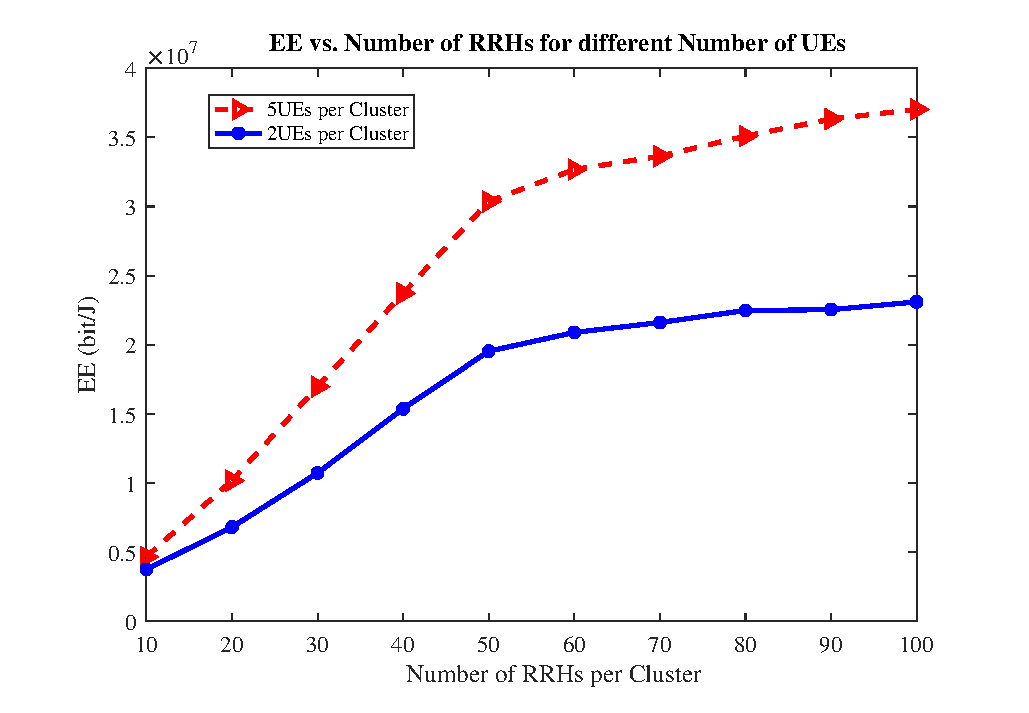
\includegraphics[width=\linewidth, height=12cm]{./fig3/rrh}
  \caption{
  بازدهی انرژی با توجه به تغییرات تعداد واحدهای رادیویی در هر خوشه برای توان بهینه برای 
   دو کاربر مختلف
   و پارامترهای جدول \ref{tab:title}}
  \label{fig:nem1}
\end{figure}
 در شکل \ref{fig:nem1}، بازدهی انرژی سیستم \lr{MIMO C-RAN} بر اساس تعداد واحدهای رادیویی در هر خوشه برای الگوریتم مورد استفاده و برای دو تعداد کاربر متفاوت، رسم شده است. 
 همانطور که  شکل  نشان می دهد، با افزایش تعداد واحدهای رادیوی، بازدهی انرژی افزایش می یابد و سپس  در این شکل از حدود 50 واحد رادیویی شیب افزایش بازدهی انرژی کمتر شده و به نظر می آید که رو به ثابت شدن است زیرا با افزایش واحد های رادیویی ابتدا نرخ ارسال داده بیشتر می شود و بازدهی انرژی بهبود می یابد و در نهایت نرخ ارسال داده دیگر بیشتر نمی گردد و ثابت می شود. زیرا در اینجا با افزایش تعداد واحدهای رادیویی، مجموع توان کل افزایش می یابد در نتیجه نرخ انتقال داده نیز بیشتر می گردد.

  \begin{figure}[h]
  \centering
    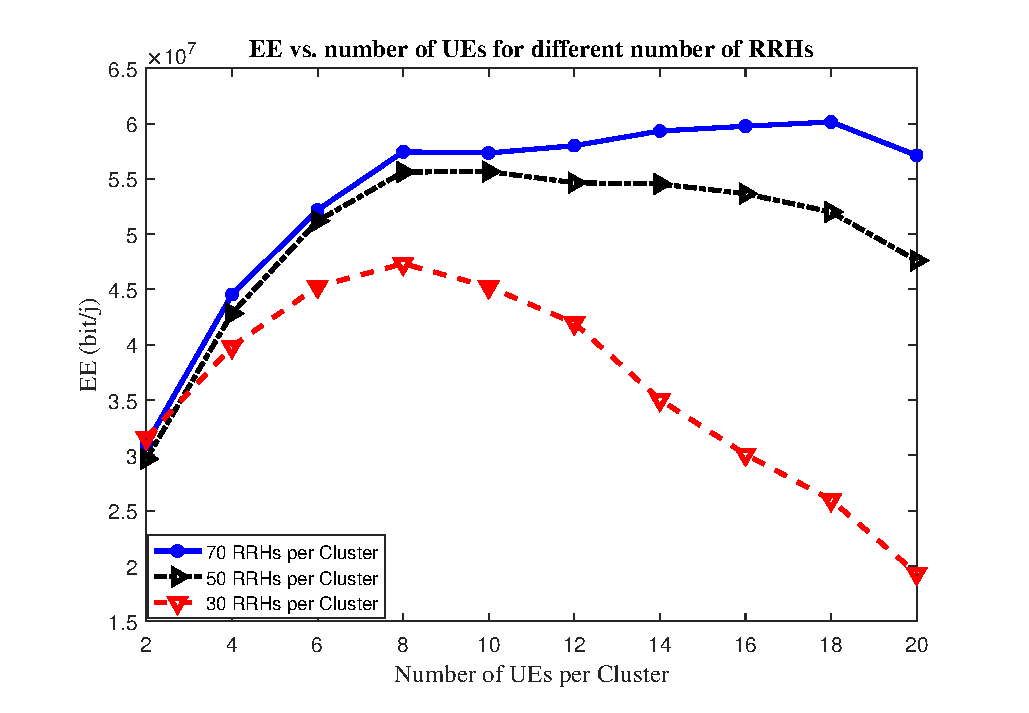
\includegraphics[width=\linewidth]{./fig3/ueEnd}
  \caption{  بازدهی انرژی با توجه به تغییرات تعداد کاربران در هر خوشه برای توان بهینه  برای 
   سه واحد رادیویی مختلف
   و پارامترهای جدول \ref{tab:title} و $P_c = 9dbm$}
  \label{fig:nem2}
\end{figure}


در شکل \ref{fig:nem2}، بازدهی انرژی بر اساس تعداد کاربران در هر خوشه برای الگوریتم مورد استفاده و برای سه تعداد واحد رادیویی متفاوت، رسم شده است.همانطور که  دیده می شود با افزایش تعداد کاربران، ابتدا شیب نمودار زیاد می شود و بازدهی انرژی افزایش می یابد زیرا با افزایش کاربران مجموع نرخ های انتقال افزایش می یابد ولی از یک مقدار به بعد تداخل بین کاربران افزایش می یابد و تاثیر خودر را به طور محسوس بر بازدهی انرژی می گذارد و در نتیجه بازدهی انرژی کاهش می یابد. 

%\bibliographystyle{ieeetr}
%\bibliography{bib1}
%\setLTRbibitems
\begin{figure}[H]
  \centering
    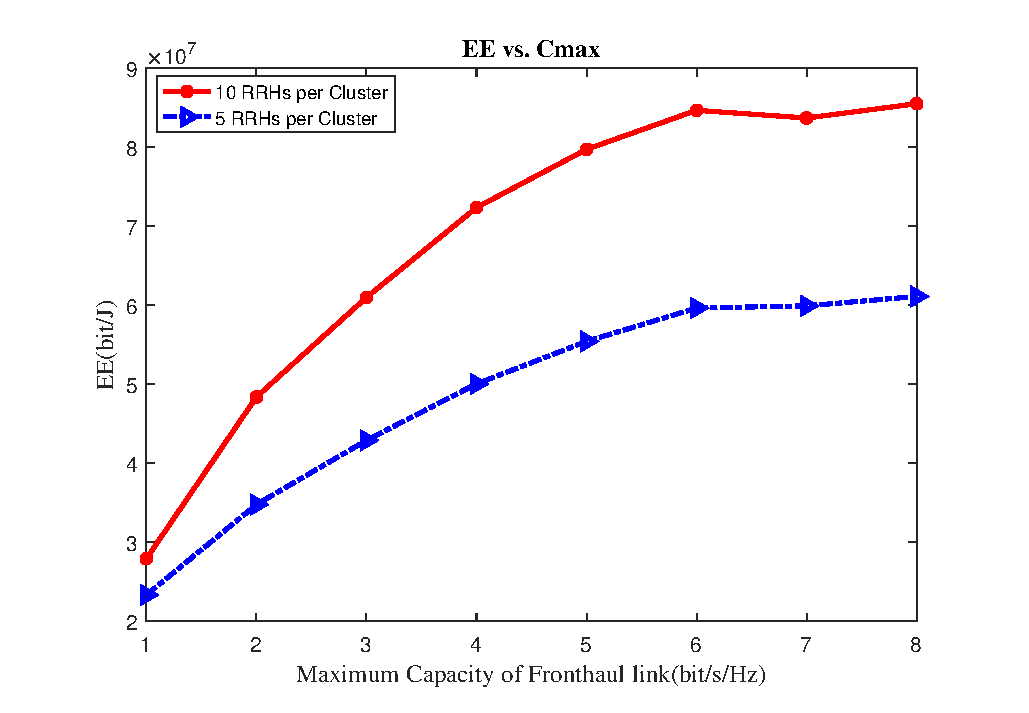
\includegraphics[width=\linewidth]{./fig3/cm}
  \caption{  بازدهی انرژی با توجه به تغییرات $C^{th}$، در در حالت $S =2$, $\text{\lr{Number of RRHs per Cluster}} = 10 , 5$, $\text{\lr{Number of UE per Cluster}} =2$ }
  \label{fig:nem3}
\end{figure}

در شکل \ref{fig:nem3}، بازدهی انرژی بر اساس محدودیت ظرفیت لینک \lr{fronthaul}، برای دو تعداد متفاوت  5 و 10 واحد رادیویی در هر خوشه رسم شده است. با توجه به شکل، زمانی که ظرفیت یک مقداری بیشتر
 می گردد، بدلیل اینکه نرخ قابل دسترس توسط تعداد کاربران و واحدهای رادیویی محدود می گردد، به نظر می آید افزایش محدودیت این ظرفیت تاثیر چندانی در بازدهی انرژی ندارد.  

% \begin{figure}[H]
%  \centering
%    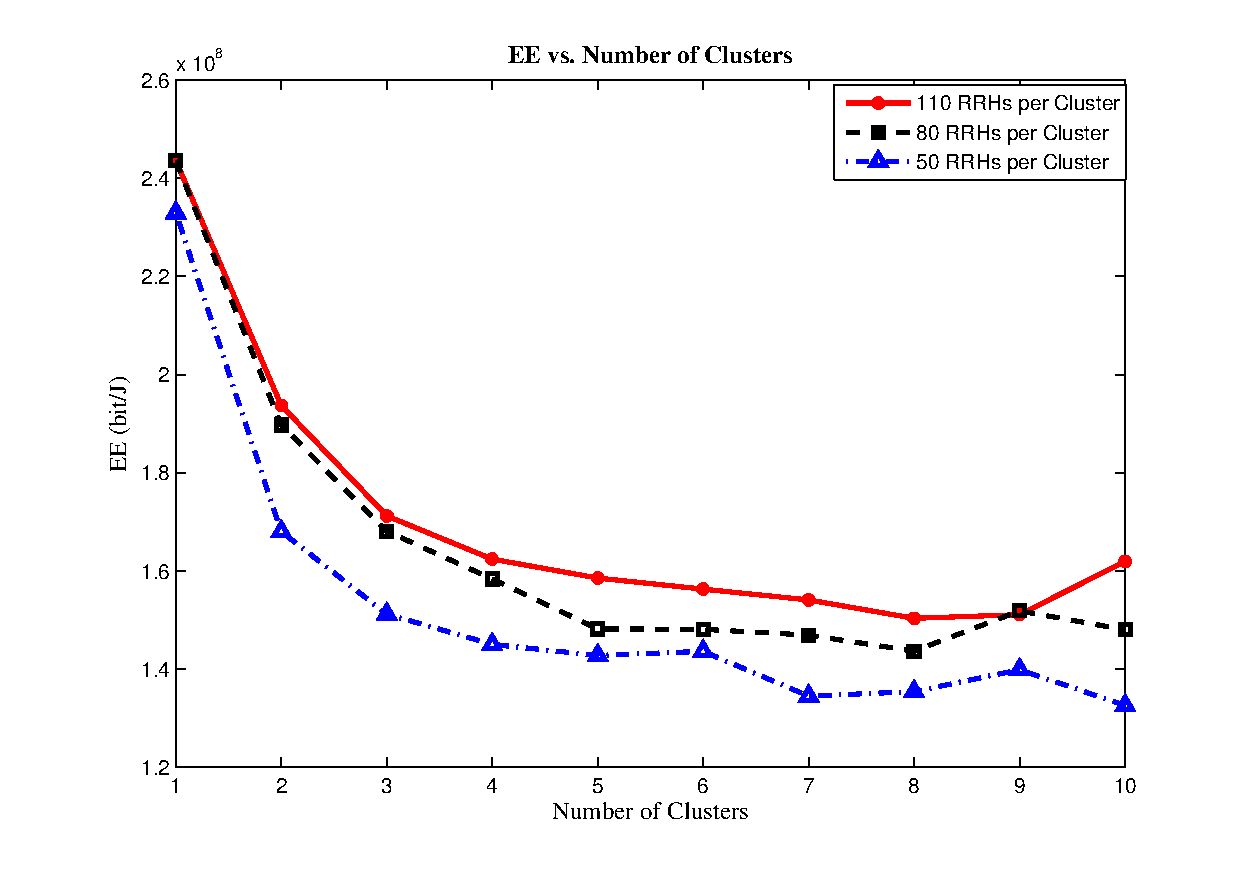
\includegraphics[width=\linewidth]{./fig3/clust}
%  \caption{  بازدهی انرژی بر حسب تعداد خوشه ها برای سه مقدار 50 و 80 و 110 واحد رادیویی}
%  \label{fig:cluster}
%\end{figure}
% حال در شکل \ref{fig:cluster}، بازدهی انرژی بر حسب تعداد خوشه ها برای سه مقدار 50 و 80 و 110 واحد رادیویی در هر خوشه با فرض وجود 3 کاربر در هر خوشه رسم شده است. همانطور که می بینید با افزایش خوشه ها بازدهی انرژی کاهش یافته است.
% 
 
 \begin{figure}[H]
  \centering
    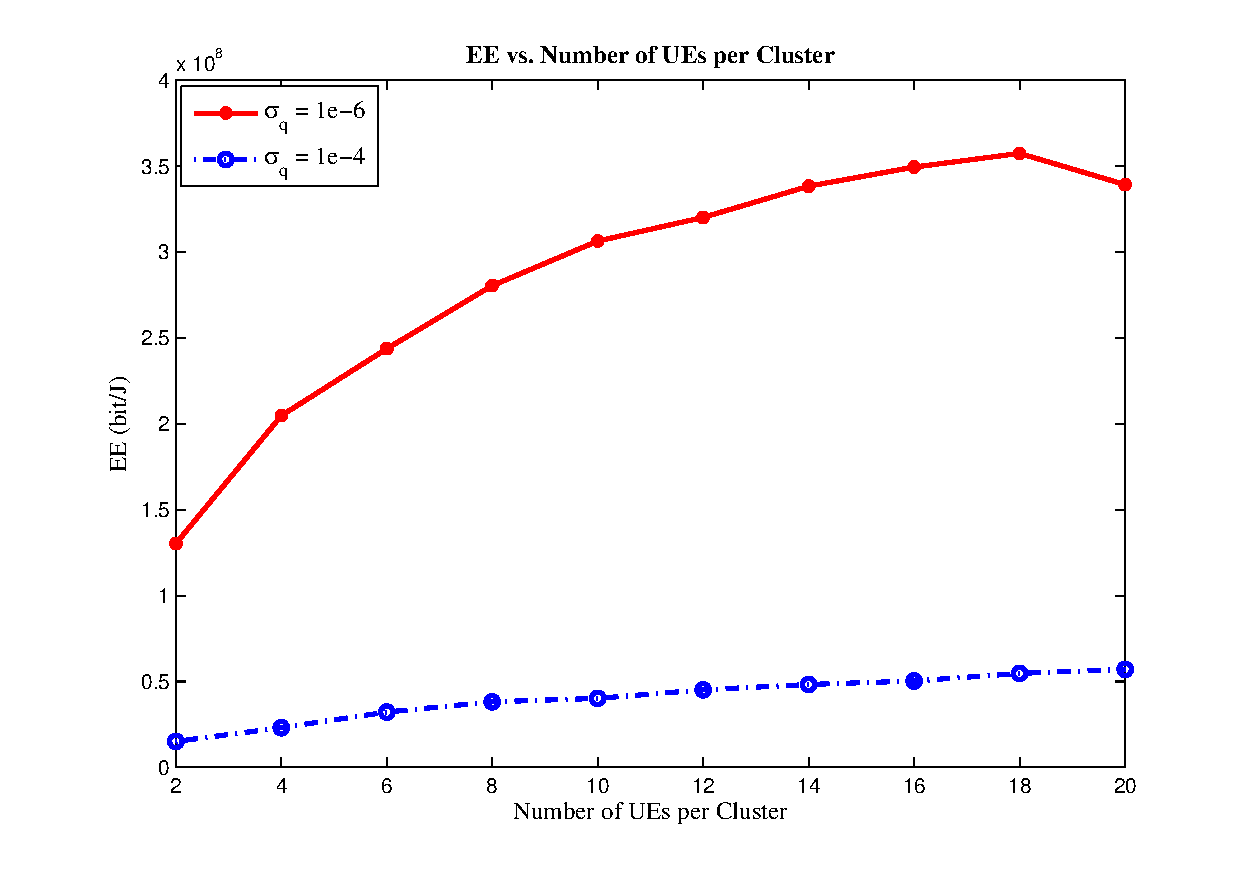
\includegraphics[width=\linewidth]{./fig3/varUE}
  \caption{  بازدهی انرژی بر حسب تعداد کاربران در 3 خوشه  برای دو مقدار 
  $\sigma_q = 1e-4 , 1e-6$
   100 واحد رادیویی
   در هر خوشه}
  \label{fig:Var}
\end{figure}
 حال در شکل \ref{fig:Var}، بازدهی انرژِی بر حسب تعداد کاربران در هر خوشه  برای برای دو مقدار 
  $\sigma_q = 10^{-4} , 10^{-6}$
   و وجود 3 خوشه در هر خوشه با فرض بودن  100 واحد رادیویی در هر خوشه رسم شده است.همانطور که می بینید با افزایش کاربران بازدهی انرژی افزایش یافته است و بازدهی انرژی در واریانس نویز کمتر بشتر از بازدهی انرژی در واریانس نویز بیشتر می باشد.
%    \begin{figure}[H]
%  \centering
%    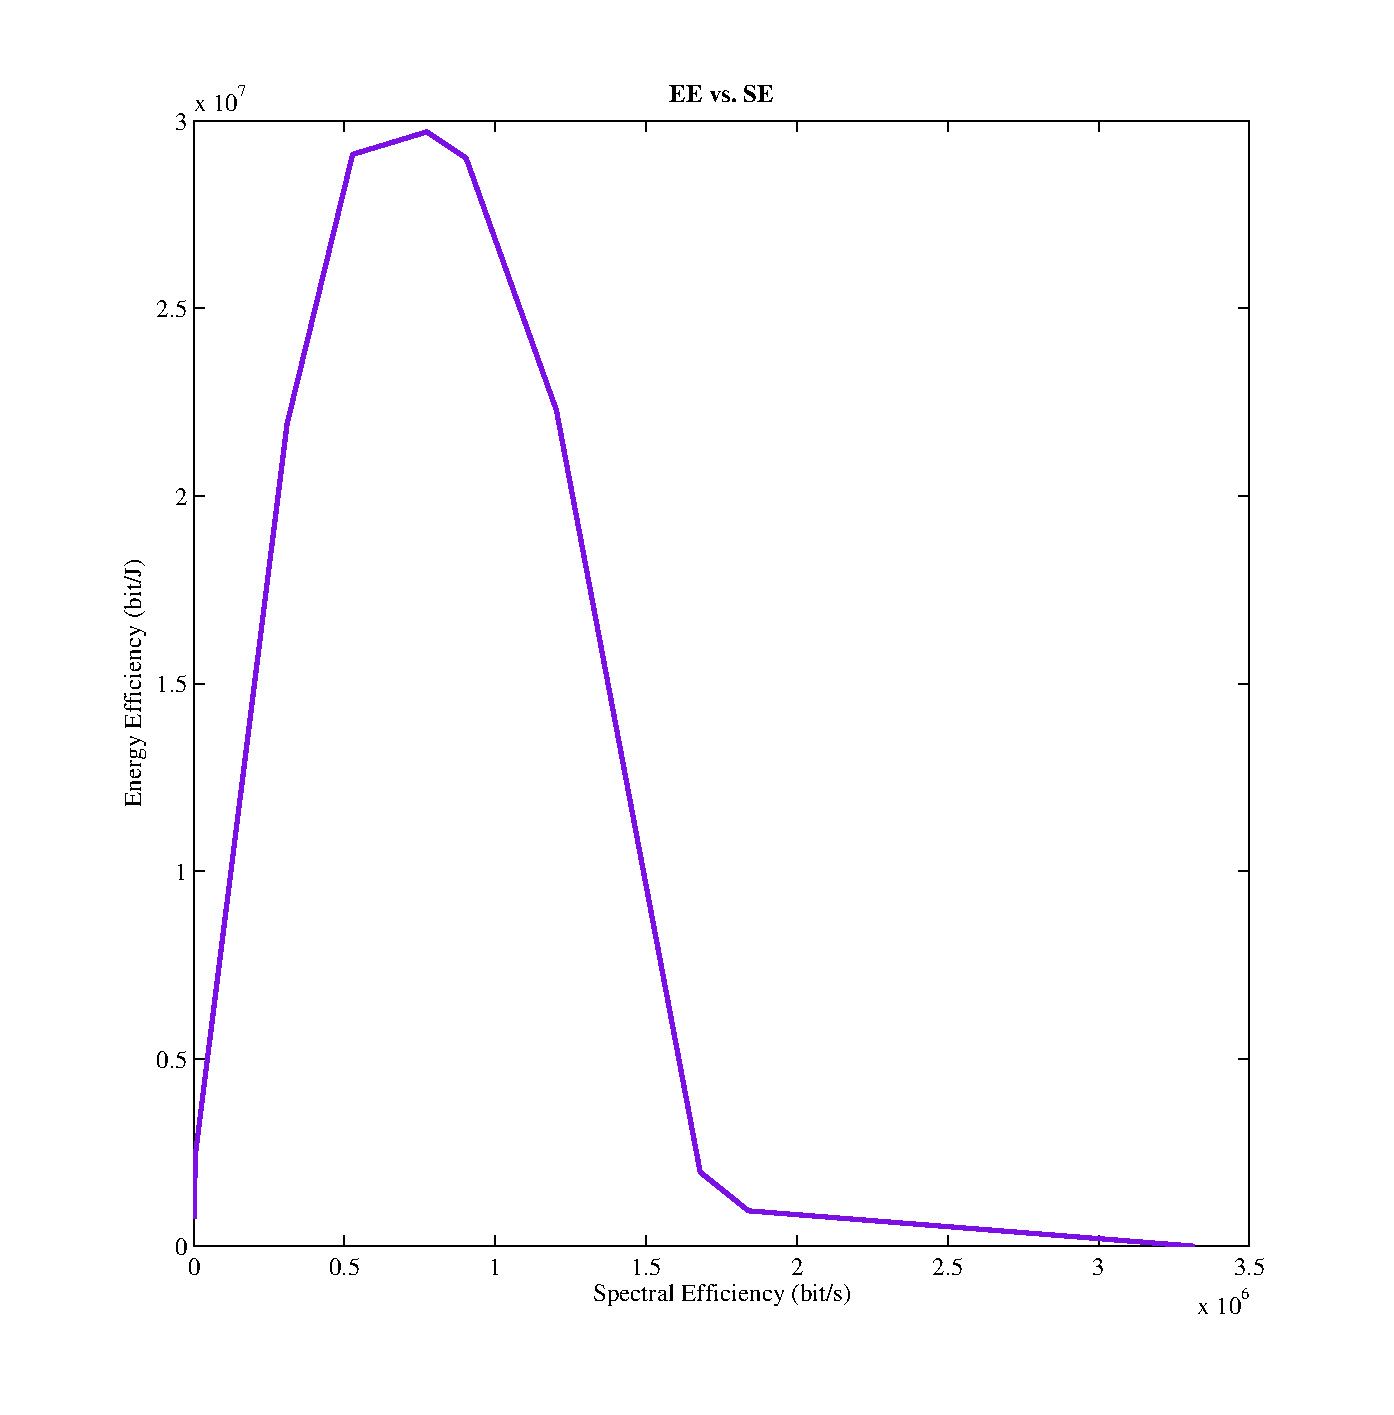
\includegraphics[width=\linewidth]{./fig3/spect}
%  \caption{  بازدهی انرژی بر حسب بازدهی طیف}
%  \label{fig:spect}
%\end{figure}
%در شکل \ref{fig:spect}، بازدهی انرژی بر حسب بازدهی طیف برای 2 خوشه که در هر خوشه 2 کاربر و 10 واحد رادیویی قرار دارد ($\sigma_q = 10^{-4}$)، رسم شده است. این نمودار با تغییر توان بیشینه ی هر واحد رادیویی رسم شده است. ابتدا با افزایش توان از مقدار 0 بازدهی انرژی بر حسب بازدهی طیف زیاد می شود و در نهایت با افزایش توان بازدهی انرژی بر حسب بازدهی طیف کاهش می یابد.  
\subsection{نتیجه گیری}
در این بخش، تخصیص توان بهینه در لینک فروسو برای مدل سیستم \lr{MIMO C-RAN} با فرض محدودیت بر روی ظرفیت \lr{fronthaul}، در نظر گرفته شده است. مدل سیستم شرح داده شده و مسئله ی تخصیص توان بهینه با روش الگوریتم بهینه و استفاده از تابع لاگرانژ حل شده است. شبیه سازی ها نشان می دهد که با افزایش تعداد واحدهای رادیویی عملکرد سیستم بهبود داده و افزایش تعداد کاربران ابتدا منجر به افزایش بازدهی انرژی می گردد و سپس به دلیل زیاد شدن تاثیر تداخل، \lr{EE} کاهش می یابد. همچنین با کاهش نویز کوانتیزاسیون عملکرد سیستم بهبود می یابد. علاوه بر این، با افزایش  بیشینه ظرفیت لینک \lr{fronthaul} ابتدا بازدهی انرژی زیاد شده سپس شیب افزایش بازدهی انرژی، کم می شود.
%%%%%%%%%%%%%%%%%%%%%%%%%%%%%%%%%%%%%%%%%%%%%%%%%
\section{لینک فراسو}
در این بخش، لینک فراسو برای سیستم \lr{MIMO C-RAN} در نظر گرفته شده است که  پیام در مسیر لینک فراسو از کاربر به واحدهای رادیویی منتقل می شود و پس از فشرده سازی توسط لینک \lr{fronthaul} به واحد کنترل منتقل می گردد. \newline
همانند لینک فروسو فرض بر این است که واحدهای رادیویی و کاربران خوشه بندی شده اند به طوری که هر خوشه  شامل تعدادی واحد رادیویی است که به کاربران موجود در آن خوشه، سرویس دهی می کنند.

 \begin{figure}
  \centering
    \includegraphics[scale = 0.45]{./fig/Drawing2}
  \caption{ساختار 
  \lr{C-RAN}
  در  لینک فراسو
  }
  \label{fig:cr2}
\end{figure}
همچنین در این مدل از روش پرتو دهی برای کاهش تداخل استفاده می کنیم که پرتو دهی در داخل واحد کنترل صورت می گیرد.
در ادامه، ابتدا سیستم  مدل و سپس نرخ قابل دسترسی بیان شده و مسئله ی تخصیص توان بررسی می گردد.
\subsection{مدل سیستم}
مدل سیستم برای لینک فراسو نیز همانند لینک فروسو می باشد که در ادامه شرح داده شده است\cite{ofdma,ulCompression}.
 سیستم \lr{MIMO C-RAN} شامل $R$ واحد رادیویی می باشد که $D$ کاربر تک آنتنه را سرویس می دهند.فرض بر این است که کاربران و واحد رادیوییها، به 
 $S$
خوشه تقسیم شده اند که $v$ امین خوشه،
 دارای $R_v$ واحد رادیویی است که ${D}_v$ کاربر را سرویس دهی می کنند.
 علاوه بر این، فرض بر این است که
$j$
امین واحد رادیویی، در $v$امین خوشه، توسط لینک فیبر نوری با ظرفیت محدود $c_{r_{(v,j)}}$ به واحد کنترل متصل می گردد.
\begin{equation}
\begin{split}
\mathcal{R}_v= \{  r_{(v,i)} | 1 \leq i \leq {R}_v , i\in Z^+\}, \\
\mathcal{C}_{\mathcal{R}_v}= \{C_{r_{(v,j)}}| 1 \leq j \leq {R}_v , j\in Z^+\}, \\
\mathcal{D}_v= \{  d_{(v,k)} | 1 \leq k \leq {D}_v , k\in Z^+\},  \\
\end{split}
\end{equation} 
که
 $\mathcal{R}_v$، $\mathcal{C}_{\mathcal{R}_v}$
 و
  $\mathcal{D}_v$
 به ترتیب نشان دهنده ی دسته واحد رادیوییها، دسته ی ظرفیت لینک \lr{Fronthaul} و دسته ی کاربران در $v$امین دسته ی خوشه می باشد.\newline
واحد رادیویی
ها تداخل پیام ها را از خوشه های دیگر نیز دریافت می کنند.\newline
 \subsection{آنالیز نرخ قابل دسترس}
در این قسمت، هدف بررسی نرخ قابل دسترسی سیستم می باشد.
\begin{theorem}\label{t1}
 نرخ قابل دسترسی برای کاربر $d_{(s,k)}$ به صورت زیر می باشد:
\begin{equation}\label{e1}
\mathfrak{R}_{d_{(s,k)}} = B \log_2(1+\gamma_{d_{(s,k)}}),
\end{equation}
که $B$ پهنای باند کانال و $\gamma_{d_{(s,k)}}$ همان \lr{SINR} دریافتی $k$امین کاربر در $s$امین دسته ی خوشه است که به صورت زیر بیان می گردد.  
\begin{equation}\label{5}
\gamma_{d_{(s,k)}}= \frac{p_{d_{(s,k)}} |{\boldsymbol{w}^H}_{\mathcal{R}_{s},d_{(s,k)}}^آ\boldsymbol{h}_{\mathcal{R}_s, d_{(s,k)}}|^2}{I_{d_{(s,k)}}+B\nu}.
\end{equation}
در فرمول \eqref{5}، 
$I_{d_{(s,k)}}$
نشان دهنده ی توان سیگنال تداخلی است.$B\nu$
نشان دهنده ی توان نویز است و
$\boldsymbol{h}_{\mathcal{R}_s, d_{(s,k)}}$ 
 نشان دهنده ی بردار کانال بین $k$امین کاربر و واحدهای رادیویی
 $s$
 امین دسته ی خوشه می باشد. همچنین 
 $\boldsymbol{w}_{\mathcal{R}_{s},d_{(s,k)}}$
 نشان دهنده ی بردار پرتو دهی استفاده شده در $s$امین دسته ی خوشه ها برروی واحدهای رادیویی برای بدست آوردن پیام $k$امین کاربر می باشد. 
 $p_{d_{(s,k)}}$
 توان ارسالی$k$امین کاربر در $s$امین دسته ی خوشه می باشد.
\end{theorem}
\begin{proof}
در این قسمت می خواهیم $\gamma$ را بدست آوریم

فرض کنید $\boldsymbol{y}_{\mathcal{R}_s}$ یک بردار
 $R_s \times 1$
باشد که نشان دهنده ی سیگنال دریافتی توسط دسته ای از واحدهای رادیویی در $s$
امین خوشه باشد که به صورت زیر بدست می آید.
\begin{equation} \label{1}
\boldsymbol{y}_{\mathcal{R}_s} = \sum_{v=1}^S \boldsymbol{H}_{\mathcal{R}_v,\mathcal{D}_s}{\boldsymbol{x}}_{\mathcal{D}_v}+ \boldsymbol{z}_{\mathcal{D}_s},
\end{equation}
که   ${\boldsymbol{x}}_{ \mathcal{D}_v} = [{x}_{ d_{(v,1)}},...,{ x}_{ d_{(v,\mathcal{D}_v)}}]^T \in \mathbb{C}^{{D}_v } $ 
بردار سمبل ارسالی خوشه ی  $v$ ام می باشد.\newline
 $\boldsymbol{z_{\mathcal{D}_s}} \backsim \mathcal{N}(0,N_0\boldsymbol{I}_{{D}_s})$ 
 نویز گوسی سفید اضافه شونده می باشد که دارای توان $N_0$
 و \newline
 $\boldsymbol{H}_{\mathcal{R}_v,\mathcal{D}_s}  \in \mathbb{C}^{{R}_v\times {D}_s}$ 
 نشان دهنده ی ماتریس کانال بین  کاربران $\mathcal{D}_s$ در دسته ی
 $s$
   ام و واحدهای رادیویی   $\mathcal{R}_v$ در دسته ی   $v$ ام می باشد.\newline
همچنین مدل کانال همانند لینک فروسو با توجه به فرمول \eqref{channel}، بدست می آید.
 حال می خواهیم پیام دریافتی توسط واحد رادیویی  $n$ ام در دسته ی $s$ ام را بدست آوریم:
 
\begin{equation} \label{100}
y_{r_{(s,n)}} = \sum_{k=1}^{D_s} h_{r_{(s,n)},d_{(s,k)}} \sqrt{p_{d_{(s,k)}}}  x_{d_{(s,k)}}
+\sum_{t=1,t\neq s}^{S} \sum_{j=1}^{D_t} h_{r_{(s,n)},d_{(t,j)}} \sqrt{p_{d_{(t,j)}}} x_{d_{(t,j)}}
 +z_{r_{(s,n)}}
\end{equation}
پیام دریافتی توسط واحد رادیویی، بعد از فشرده سازی به صورت زیر می شود
\begin{equation}
\hat{y}_{r_{(s,n)}} = y_{r_{(s,n)}} + q_{r_{(s,n)}} 
\end{equation}
پیام هر کاربر در واحد کنترل با اعمال پرتو دهی \LTRfootnote{beamforming} به صورتی که در ادامه بیان شده، بدست می آید

\begin{equation}
\begin{split}
\hat{x}_{d_{(s,k)}} = & {\boldsymbol{w}^H}_{\mathcal{R}_s, d_{(s,k)}} \boldsymbol{h}_{\mathcal{R}_s, d_{(s,k)}} \sqrt{p_{d_{(s,k)}}}  x_{d_{(s,k)}} \\
+ & \sum_{i=1,i\neq k}^{D_s}  {\boldsymbol{w}^H}_{\mathcal{R}_s, d_{(s,k)}} \boldsymbol{h}_{\mathcal{R}_s, d_{(s,i)}} \sqrt{p_{d_{(s,i)}}}  x_{d_{(s,i)}} \\
+&  \sum_{t=1,t\neq s}^{S} \sum_{j=1}^{D_t} {\boldsymbol{w}^H}_{\mathcal{R}_s, d_{(s,k)}} \boldsymbol{h}_{\mathcal{R}_s, d_{(t,j)}} \sqrt{p_{d_{(t,j)}}}  x_{d_{(t,j)}} \\
+& {\boldsymbol{w}^H}_{\mathcal{R}_s, d_{(s,k)}}  ({\boldsymbol{q}}_{\mathcal{R}_s} + {\boldsymbol{z}}_{\mathcal{R}_s})
\end{split}
\end{equation}
حال برای بدست آوردن  \lr{SINR}، توان سیگنال بر روی توان تداخل و نویز را بدست می آوریم:
\begin{equation}
\gamma = \frac{p_{d_{(s,k)}}|{\boldsymbol{w}^H}_{\mathcal{R}_s, d_{(s,k)}} \boldsymbol{h}_{\mathcal{R}_s, d_{(s,k)}}|^2}{
  I_{d_{(s,k)}}
+ B \times \nu_{d_{(s,k)}}
}
\end{equation}
که داریم :
\begin{equation}
\begin{split}
\nu_{d_{(s,k)}}&  = {\boldsymbol{w}^H}_{\mathcal{R}_s, d_{(s,k)}}  (diag({\sigma_n^2}_{r_{(s,1)}}...{\sigma_n^2}_{r_{(s,R_s)}})+diag({\sigma_q^2}_{r_{(s,1)}}...{\sigma_q^2}_{r_{(s,R_s)}})) {\boldsymbol{w}}_{\mathcal{R}_s, d_{(s,k)}}\\
I_{d_{(s,k)}}& = \sum_{i=1,i\neq k}^{D_s}  |{\boldsymbol{w}^H}_{\mathcal{R}_s, d_{(s,k)}} \boldsymbol{h}_{\mathcal{R}_s, d_{(s,i)}}|^2 p_{d_{(s,i)}} +\sum_{t=1,t\neq s}^{S} \sum_{j=1}^{D_t} |{\boldsymbol{w}^H}_{\mathcal{R}_s, d_{(s,k)}} \boldsymbol{h}_{\mathcal{R}_s, d_{(t,j)}}|^2 p_{d_{(t,j)}} 
\end{split}
\end{equation}
 در اینجا  $\sigma_n^2$ واریانس نویز می باشد که  برای سادگی برای همه ی واحدهای رادیویی ثابت فرض شده و  دارای مقدار $N_0$ 
است و $\sigma_q^2$ واریانس نویز فشرده سازی می باشد.
علاوه بر این با استفاده از پرتودهی \lr{MMSE}، ماتریس پرتودهی به صورت زیر است 
\begin{equation}
\boldsymbol{W}_{\mathcal{R}_s,\mathcal{D}_s} = \hat{\boldsymbol{H}}_{\mathcal{R}_s,\mathcal{D}_s}(\hat{\boldsymbol{H}}_{\mathcal{R}_s,\mathcal{D}_s}^H \hat{\boldsymbol{H}}_{\mathcal{R}_s,\mathcal{D}_s}+ \alpha \boldsymbol{I}_{{D}_s})^{-1},
\end{equation} 
همچنین  $\alpha$، فاکتور رگولاریزاسیون است در صورتی که $\alpha$ صفر یاشد، ماتریس پرتو دهی \lr{ZF} خواهیم داشت.
\end{proof}
\subsection{بهینه سازی تخصیص توان}
در این قسمت می خواهیم توان را طوری اختصاص دهیم تا بازدهی انرژی به بیشینه مقدار خود برسد.
می دانیم نرخ قابل دسترس بر روی لینک \lr{fronthaul}، بین $n$ امین واحد رادیویی در $s$ امین خوشه  و  واحد کنترل به صورت زیر بدست می آید 
\begin{equation}
C_{r_{(s,n)}} = \log{\frac{1+( \sum_{k=1}^{D_s}|h_{r_{(s,n)},d_{(s,k)}}|^2{p_{d_{(s,k)}}} + \sum_{t=1,t\neq s}^{S}\sum_{l=1}^{D_t}|h_{r_{(s,n)},d_{(t,l)}}|^2{p_{d_{(t,l)}}}+ B N_0) }{ \sigma_{q_{(s,n)}}^2})},
\end{equation}
\subsubsection{شرح مسئله}
 همانطور که گفته شد نسبت مجموع نرخ ها در سیستم به کل توان ارسالی کاربرها نشان دهنده ی بازدهی انرژی است که با $\eta$ نمایش داده می شود و می توان اینگونه بیان کرد
\begin{equation}\label{eta1}
\eta(\boldsymbol{P}) := \frac{\sum\limits_{s=1}^{S} \sum\limits_{k=1}^{{D}_s}\mathfrak{R}_{d_{(s,k)}} }{\sum\limits_{s=1}^{S} \sum\limits_{k=1}^{{K}_s}{p}_{d_{(s,k)}}} = \frac{R_{total}(\boldsymbol{P})}{P_{UE}(\boldsymbol{P})},
\end{equation}
که در اینجا  $ \boldsymbol{P} = \{ \boldsymbol{P}_{\mathcal{D}_s}|  1 \leq s \leq S, s \in \mathbb{Z}^{+} \}$ ماتریس تخصیص توان است. در این بخش، بیشینه سازی بازدهی انرژی با شروط زیر مورد بررسی قرار می گیرد 
\begin{equation}\label{p11}
\begin{aligned}
\max\limits_{\boldsymbol{P}}   \quad &   \eta(\boldsymbol{P})\\
\text{\lr{subject to}} \quad  &  0 \leq {p}_{d_{(s,k)}} \leq P_{max} && \qquad \forall s, \forall k,   \\
&\mathfrak{R}_{d_{(s,k)}} \geq  \mathfrak{R}_{d_{(s,k)}}^{th} && \qquad \forall s, \forall k, \\ 
&C_{r_{(s,i)}} \leq C_{r_{(s,i)}}^{th}  &&\qquad \forall s, \forall i, \\
\end{aligned}			
\end{equation}
همانند لینک فروسو، بدلیل محدب نبودن مسئله از روش الگوریتم تکرار شونده استفاده می کنیم.
\subsection{روش مورد استفاده}
در این قسمت، به جای ماکسیمم کردن \eqref{eta1}، همانند لینک فروسو، از قضیه ی \eqref{t2} استفاده می نماییم.
 همچنین کران بالایی برای تداخل بدست می آید که در ادامه بیان می شود.
\begin{equation} \label{id}
\tilde{I}_{d_{(s,k)}} = \sum_{v=1}^{S}  |{\boldsymbol{w}^H}_{\mathcal{R}_s, d_{(s,k)}} \boldsymbol{h}_{\mathcal{R}_v, d_{(s,i)}}|^2 P_{max} 
\end{equation}
در نتیجه با توجه به رابطه ی  \eqref{id}، می توان $\gamma$ را به این صورت تخمین زد:
\begin{equation}
\tilde{\gamma}_{d_{(s,k)}}= \frac{p_{d_{(s,k)}} |{\boldsymbol{w}^H}_{\mathcal{R}_{s},d_{(s,k)}}^آ\boldsymbol{h}_{\mathcal{R}_s, d_{(s,k)}}|^2}{\tilde{I}_{d_{(s,k)}}+B\nu}.
\end{equation}
ابتدا تابع لاگرانژ را تشکیل می دهیم تا بتوان با استفاده از آن، از الگوریتم تکرار شونده ی \eqref{alg}، استفاده کرد. 
\begin{equation}
\begin{split}
\mathcal{L}(\boldsymbol{P}; \boldsymbol{\lambda}, \boldsymbol{\mu}, \boldsymbol{ \kappa}) & = \sum\limits_{s=1}^{S} \sum\limits_{k=1}^{\mathcal{D}_s}\mathfrak{\tilde{R}}_{d_{(s,k)}} 
- \eta \sum\limits_{s=1}^{S} \sum\limits_{k=1}^{\mathcal{K}_s}{p}_{d_{(s,k)}}\\
&+\sum\limits_{s=1}^{S} \sum\limits_{k=1}^{\mathcal{D}_s} \lambda_{d_{(s,k)}} (\mathfrak{\tilde{R}}_{d_{(s,k)}}-\mathfrak{R}_{d_{(s,k)}}^{th})\\
&- \sum\limits_{s=1}^{S} \sum\limits_{k=1}^{\mathcal{K}_s} \mu_{d_{(s,k)}} ({p}_{d_{(s,k)}}-P_{max})\\
&- \sum\limits_{s=1}^{S} \sum\limits_{i=1}^{\mathcal{R}_s} \kappa_{r_{(s,i)}} (C_{r_{(s,i)}}-C_{r_{(s,i)}}^{th}).\\
\end{split}
\end{equation}
که در اینجا، $\boldsymbol{\lambda}, \boldsymbol{\mu}, \boldsymbol{\kappa} \geq 0$
بردارهای ضرایب لاگرانژ می باشد .\newline
با استفاده از این معادله و مشتقگیری از آن، توان بهینه به صورت زیر بدست می آید
\begin{equation}
p_{d_{(s,k)}}^* \approx [\frac{ B(1+\lambda_{d_{(s,k)}} )-(\sum_{n=1}^{\mathcal{R}_s}\kappa_{r_{(s,i)}})}{\ln2 \times (\eta + \mu_{d_{(s,k)}})}]^+;
\end{equation} 

  در آخر، برای بدست آوردن توان بهینه، الگوریتم \eqref{alg1} مورد استفاده قرار می گیرد \cite{hcranEE}
 \begin{latin}
\begin{algorithm}
\caption{Energy-Efficient Power Allocation}\label{alg1}
\begin{algorithmic}

\State Set the maximum number of iterations $I_{max}$, convergence condition $\epsilon_{\eta}$  and the initial value $\eta^{(1)} = 0$
\State Set the iteration index $i = 1$ and begin the iteration (Outer
Loop).
\For {$ 1\leq i \leq  Imax$}
\State Solve the resource allocation problem with $\eta^{(i)}$ (Inner Loop);
\State Obtain $P^{(i)}, R_{total}^{(i)}, P_{UE}^{(i)}$
\If {$ R_{total}(\boldsymbol{P}^{(i)}) - \eta^{(i)} P_{UE}(\boldsymbol{P}^{(i)}) < \epsilon_{\eta} $} 
\State Set $\boldsymbol{P}^*= \boldsymbol{P}^{(i)} $   and  $ \eta^{*} =\eta^{(i)} $;
\State break;
\Else
\State Set $\eta^{(i)}= \frac{R_{total}(\boldsymbol{P}^{(i))}}{P_{UE}(\boldsymbol{P}^{(i))}}$ and $i= i+1$;
\EndIf 
\State \textbf{end if}
\EndFor 
\State \textbf{end for}

\end{algorithmic}
\end{algorithm}
\end{latin}
\subsection{نتایج عددی}
در این بخش، نتایج عددی الگوریتم مورد استفاده را برای سیستم \lr{MIMO C-RAN} با پارامترهای بیان شده در جدول \ref{tab:title3} و استفاده از پرتو دهی \lr{ZF} بیان می شود.
\begin{latin} 
 \begin{table}[H]
 \caption {\rl{پارامترهای شبیه سازی}} \label{tab:title3} 
 \begin{center}
  \begin{tabular}{||c c ||} 
  \hline
  Parameter & Value \\ [0.5ex] 
  \hline\hline
  Number of cluster S & 3 \\ 
  \hline
  Noise power density & -174dBm/Hz\\
  \hline
  Bandwidth & 120KHz \\
  \hline
 Maxmimun transmit Power & 10dBm \\
  \hline
  Circuit Power of whole RRHs & 10dBm \\
  \hline
  Variance of quantization noise & $10^{-2}$ \\
  \hline
   Maxmimun fronthaul link's rate & 20bits/sec/Hz \\
  \hline
  Minimum data rate &  1bits/sec/Hz \\ [1ex] 
  \hline
 \end{tabular}
 \end{center}
 \end{table}
 \end{latin}
  \begin{figure}[H]
  \centering
    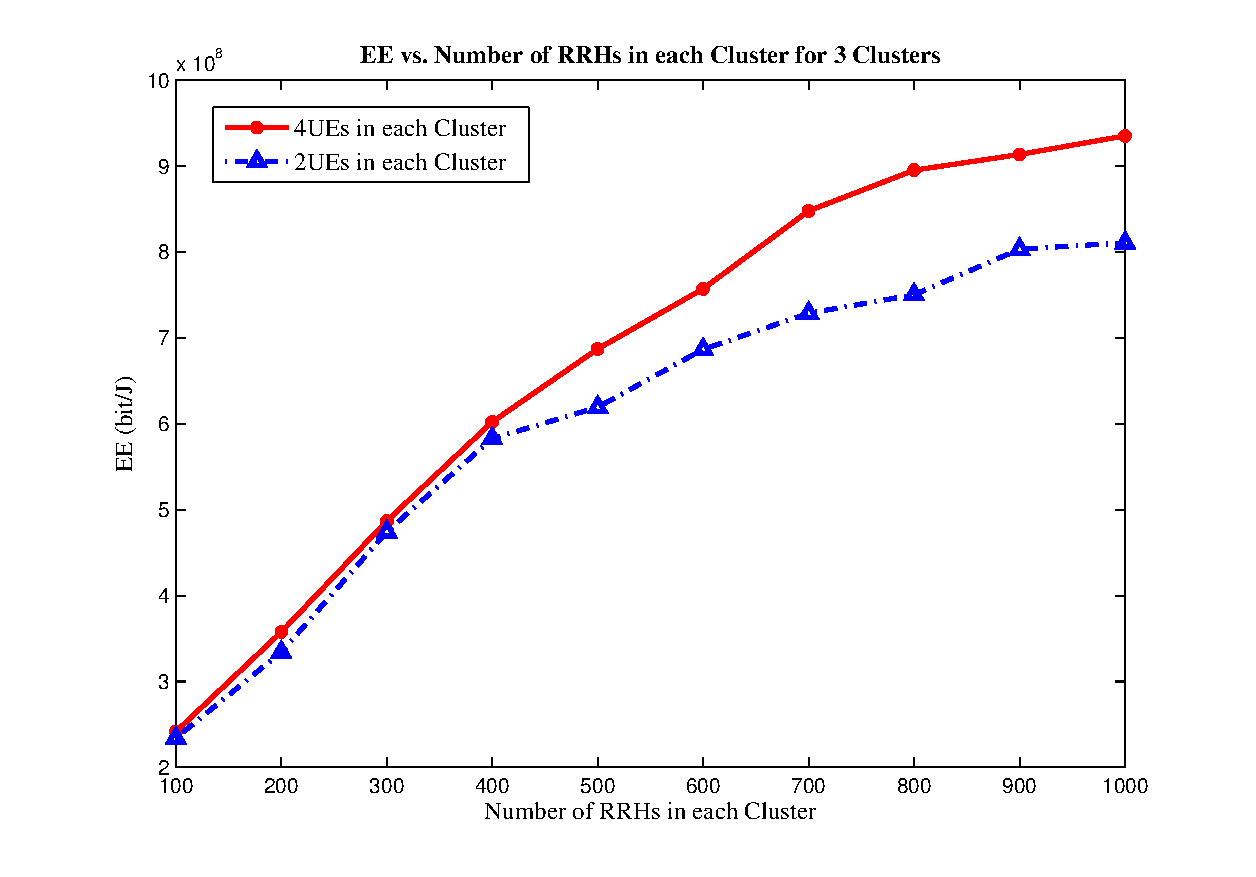
\includegraphics[width=\linewidth, height=12cm]{./fig3/rrhul}
  \caption{
  بازدهی انرژی با توجه به تغییرات تعداد واحدهای رادیویی  در هر خوشه برای توان بهینه  برای 
   دو کاربر مختلف
   و پارامترهای جدول \ref{tab:title3}}
  \label{fig:rrhul}
\end{figure}
 در شکل \ref{fig:rrhul}، بازدهی انرژی سیستم \lr{MIMO C-RAN} بر اساس تعداد واحدهای رادیویی در هر خوشه برای الگوریتم مورد استفاده و برای دو تعداد کاربر متفاوت، رسم شده است. 
 همانطور که  شکل  نشان می دهد، با افزایش تعداد واحدهای رادیوی، بازدهی انرژی افزایش می یابد و از یک مقدار به بعد شیب افزایش بازدهی انرژی کمتر شده است. زیرا با افزایش تعداد واحدهای رادیویی، مجموع توان کل افزایش یافته و در نتیجه نرخ انتقال داده نیز بیشتر می گردد.

 \begin{figure}[H]
  \centering
    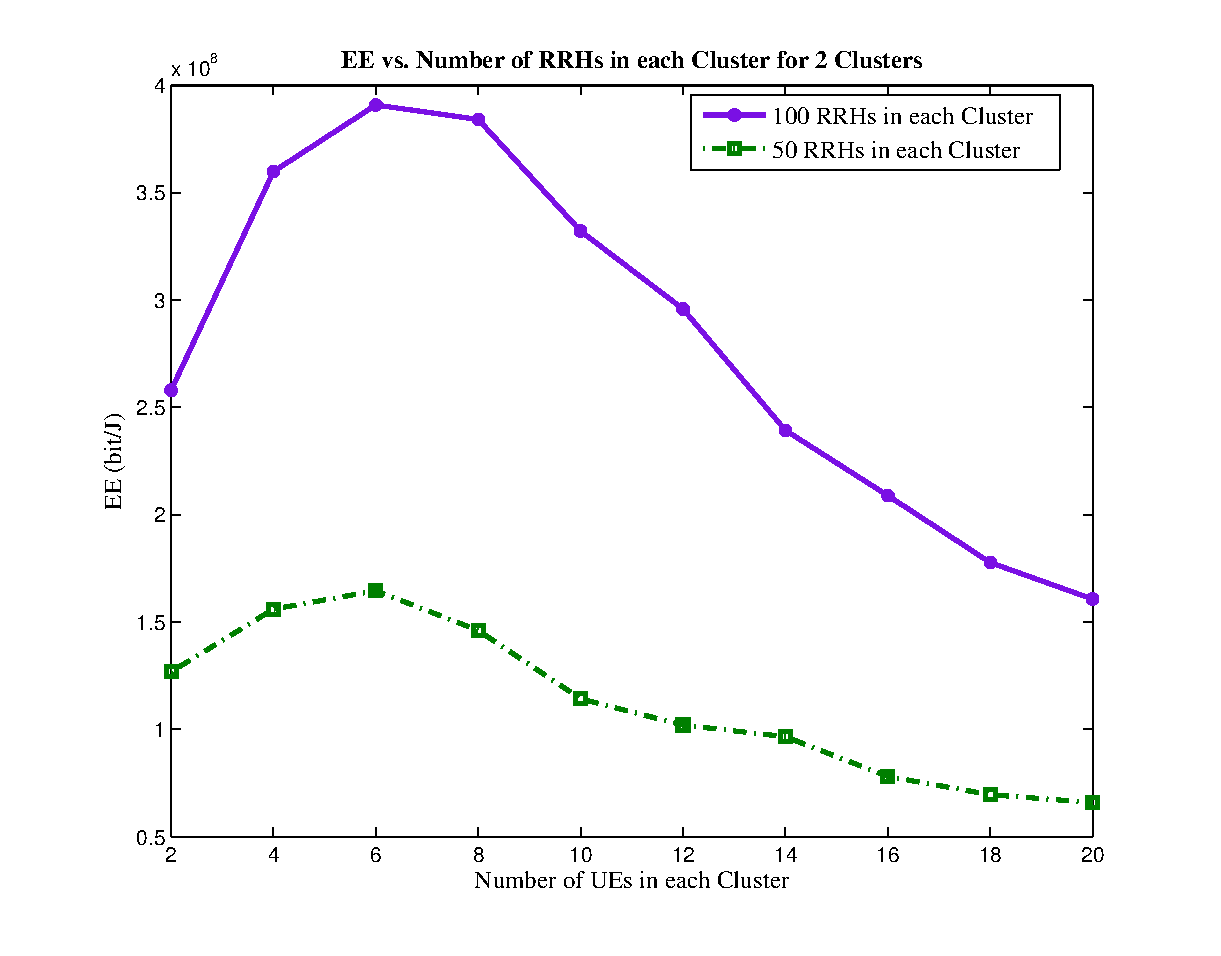
\includegraphics[width=\linewidth]{./fig3/ueul}
  \caption{  بازدهی انرژی با توجه به تغییرات تعداد کاربران در هر خوشه برای توان بهینه برای 
   دو واحد رادیویی مختلف
   و پارامترهای جدول \ref{tab:title3} و $S=2$}
  \label{fig:ueul}
\end{figure}


در شکل \ref{fig:ueul}، بازدهی انرژی بر اساس تعداد کاربران در هر خوشه برای الگوریتم مورد استفاده و برای دو تعداد واحد رادیویی متفاوت، رسم شده است. همانطور که  دیده می شود با افزایش تعداد کاربران، ابتدا شیب نمودار زیاد می شود و بازدهی انرژی افزایش می یابد سپس به دلیل افزایش تاثیر تداخل بین کاربران بازدهی انرژی کاهش می یابد. 

\begin{figure}[H]
  \centering
    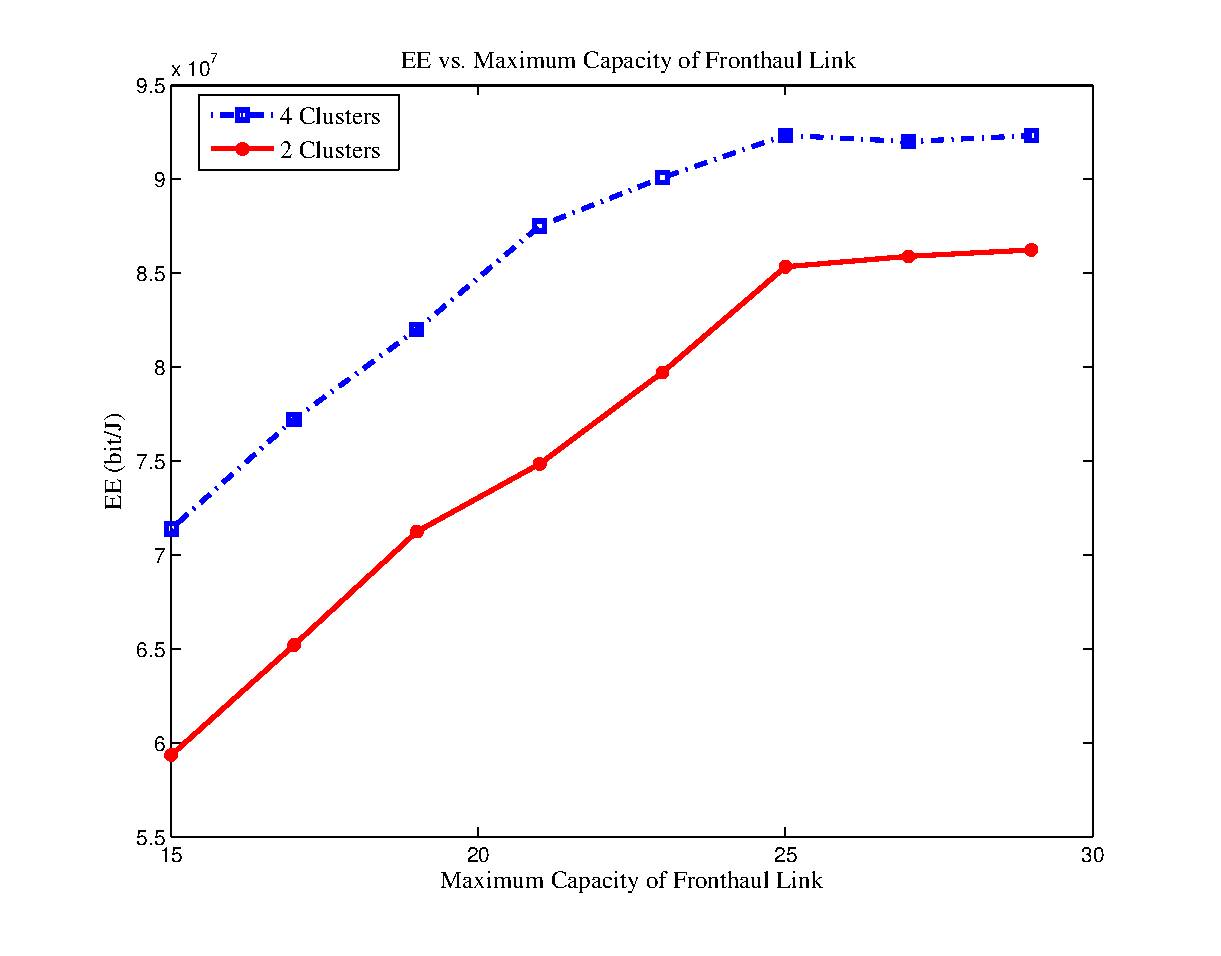
\includegraphics[width=\linewidth]{./fig3/cap}
  \caption{  بازدهی انرژی با توجه به تغییرات $C^{th}$، در در حالت $S =2 ,4 $, $\text{\lr{Number of RRHs per Cluster}} = 30$, $\text{\lr{Number of UE per Cluster}} =2$ }
  \label{fig:cap}
\end{figure}

در شکل \ref{fig:cap}، بازدهی انرژی بر اساس محدودیت ظرفیت لینک \lr{fronthaul}، برای دو تعداد متفاوت  2 و 4 خوشه و در هر خوشه 2 کاربر و 30 واحد رادیویی رسم شده است. با توجه به شکل، ابتدا با بازدهی انرژی، افزایش یافته،
سپس بدلیل اینکه نرخ قابل دسترس توسط تعداد کاربران و واحدهای رادیویی محدود می گردد، به نظر می آید افزایش محدودیت این ظرفیت تاثیر چندانی در بازدهی انرژی ندارد.  
\subsection{نتیجه گیری}
در این بخش، تخصیص توان بهینه در لینک فراسو برای مدل سیستم \lr{MIMO C-RAN} با فرض محدودیت بر روی ظرفیت \lr{fronthaul} و وجود چندین خوشه، در نظر گرفته شده است. مدل سیستم  شرح داده شده و مسئله ی تخصیص توان بهینه با روش الگوریتم بهینه و استفاده از تابع لاگرانژ حل شده است. شبیه سازی ها نشان می دهد همانند لینک فروسو با افزایش تعداد واحدهای رادیویی عملکرد سیستم بهبود داده و افزایش تعداد کاربران منجر به افزایش بازدهی انرژی می گردد ولی در نهایت به دلیل تداخل بازدهی انرژی کاهش می یابد. همچنین، با افزایش  بیشینه ظرفیت لینک \lr{fronthaul} ابتدا بازدهی انرژی زیاد شده سپس شیب افزایش بازدهی انرژی، کم می شود.
%%%%%%%%%%%%%%%%%%%%%%%%%%%%%%%%%%%%%%%%%%%%%%